

\chapter{Background}\label{chapter:background}

\section{Dynamic Scene Graph for Video}
The scene graph is a structured representation of a scene that can clearly express the objects, attributes, and relationships between objects in the scene\cite{9661322}. Accompanied by the development of computer vision technology, simply detecting and recognizing objects in images no longer satisfies the researchers, as they would expect some higher level of understanding and reasoning for image vision tasks. In this way, an intuitive idea comes up about adding up the relationship between the detected objects(See example in figure \ref{fig:SGG}). The earliest research could dated back to 2017, when some objects and relations of a given image could be inferred and a scene graph would be produced as a result\cite{xu2017scene}. Other research like Neural Motifs\cite{zellers2018neural} also shows the possibility of predicting the most frequent relation between object pairs with the given labels and object detections. Later in 2018, videos came into discussion, and both spatial and temporal relations would be concerned in the dynamic graph researchers propose to represent\cite{wang2018videos}. Meanwhile, the accuracy of Scene Graph Detection tasks has significantly improved thanks to the application of unbiased SGG\cite{wang2018videos}, fueled by the \textbf{Detection2} \cite{wu2019detectron2}, a library that contains various state-of-the-art detection and segmentation algorithms. In a nutshell, representing videos as dynamic scene graphs including the detection of objects and the relations in between has been realized in the past years. And our work would utilize such technique and extract our driver-oriented dynamic scene graphs for further learning.

\begin{figure}
    \centering
    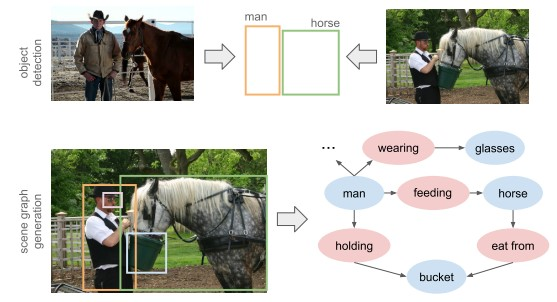
\includegraphics[width=0.8\linewidth]{figures/SGG.jpg}
    \caption{Scene Graph Generation by Iterative Message Passing}
    \label{fig:SGG}
\end{figure}


\section{Large Language Model}
Large Language Models (LLMs) are highly complex artificial intelligence systems that can learn from the vast amounts of available text data\cite{radford2018improving}. Thanks to the attending of \textit{Transformer} \cite{vaswani2017attention}, a deep learning architecture, these language models which employed self-supervised pre-training have demonstrated improved efficiency and scalability in many fields.
 Based on self-attention mechanisms and feed-forward module,\textit{Transformer} has overwhelming advantages in computing representations and global dependencies.

In concrete terms, the Large Language Models equipped with \textit{Transformer} are capable of diverse tasks raised by Natural Language Processing\cite{chowdhary2020natural}, such as textual entailment, question answering, semantic similarity assessment, and document classification. Take BERT\cite{alaparthi2020bidirectional} and GPT \cite{radford2018improving,radford2019language,brown2020language} as two examples, the former utilizes transformer encoder blocks to predict missing words in a given text, and the latter has been enjoying a tremendous reputation for generating diverse and human-like responses, showcasing its potential in various domains.

    \subsection{Text Classification}
In our project, a bunch of hierarchical activity labels would be acquired from the dataset \textit{drive \& act} to depict every detail of the participant's movements in the driving behavior recorded in the video. These labels, however, are too trivial for the construction of learning data, as considering each activity individually will be tedious in such a vast and complex model training process. Therefore, labels should be classified according to the object on which this behavior operates or the specificity of the moment in which the action takes place. For example, the fastening of a seat belt should occur shortly after entering the vehicle, and all behavior related to eating or drinking should be classified into the same group.

In our task, we use zero-shot text classification. This is a task where a model is trained on a set of labeled examples and then classifies new examples from previously unseen classes. This method, which leverages a pre-trained language model, can be thought of as an instance of transfer learning which generally refers to using a model trained for one task in a different application than what it was originally trained for. This is particularly useful for situations where the amount of labeled data is small, for example, our work with 39 different behaviors to be classified.

The model used in the pipeline is \textit{BART} \cite{lewis2019bartdenoisingsequencetosequencepretraining}. According to the paper, BART is trained by corrupting text with an arbitrary noising function and learning a model to reconstruct the original text. It uses a standard Tranformer-based neural machine translation architecture which, despite its simplicity, can be seen as generalizing BERT (due to the bidirectional encoder), GPT (with the left-to-right decoder), and many other more recent pretraining schemes. With all these prerequisites it is quite obverious that \textit{BART} is a very practical model for our classification task.

\section{graph}




    \subsection{Dynamic graph}

    \subsection{Graph Neural Networks}

\section{behavior prediction}

